\ifdefined\ishandout
\documentclass[handout]{beamer}
\else
\documentclass{beamer}
\fi

\usepackage[frenchb]{babel}
\usepackage[T1]{fontenc}
\usepackage[latin1]{inputenc}
\usepackage{hyperref}
\usepackage{multirow}
\usepackage{listings}
\usepackage{fancyvrb}
\usepackage{tikz}
\usepackage{framed}
\usepackage{algorithm}
\usepackage{algorithmic}
\usepackage{xcolor}
\usepackage{color, colortbl}
\ifdefined\ishandout
\usepackage{handoutWithNotes}
\fi
\usepackage{amsmath}
\usepackage{bm}
\usepackage{hhline}

\usetikzlibrary{shapes.geometric}
\usetikzlibrary{positioning}
\usetikzlibrary{shapes.arrows, chains}
\usetikzlibrary{arrows,calc}
\usetikzlibrary{shapes.multipart}
\usepackage{array}
\usetheme{Boadilla}

\usefonttheme[onlymath]{serif}

\newcommand{\R}{\mathbb{R}}
\newcommand{\C}{\mathbb{C}}
\newcommand{\N}{\mathbb{N}}
\newcommand{\Z}{\mathbb{Z}}
\newcommand{\E}{\mathbb{E}}
\newcommand{\Var}{\text{Var}}
\newcommand{\Cov}{\text{Cov}}
\ifdefined\ishandout
\pgfpagesuselayout{3 on 1 with notes}[a4paper,border shrink=5mm]
\usecolortheme{dove}
\else
%\usecolortheme{dolphin}
\usecolortheme{beaver}
\fi


\lstnewenvironment{codeC}
{ \lstset{language=C,
    otherkeywords={printf,scanf}}
}
{}

\ifdefined\ishandout
\definecolor{mygreen}{rgb}{0,0,0}
\definecolor{mymauve}{rgb}{0,0,0}
\definecolor{myblue}{rgb}{0,0,0}
\else
\definecolor{mygreen}{rgb}{0,0.6,0}
\definecolor{mymauve}{rgb}{0.58,0,0.82}
\definecolor{myblue}{rgb}{0,0,1}

\fi

%% Notes
%\setbeameroption{show only notes}


\definecolor{mygray}{rgb}{0.5,0.5,0.5}

\lstset{ language=Python,%
  backgroundcolor=\color{white},   % choose the background color; you must add \usepackage{color} or \usepackage{xcolor}
  basicstyle=\footnotesize,        % the size of the fonts that are used for the code
  breakatwhitespace=false,         % sets if automatic breaks should only happen at whitespace
  breaklines=true,                 % sets automatic line breaking
  captionpos=b,                    % sets the caption-position to bottom
  commentstyle=\color{mygreen},    % comment style
  deletekeywords={...},            % if you want to delete keywords from the given language
  escapeinside={\%*}{*)},          % if you want to add LaTeX within your code
  extendedchars=true,              % lets you use non-ASCII characters; for 8-bits encodings only, does not work with UTF-8
  frame=tb,	                   % adds a frame around the code
  keepspaces=true,                 % keeps spaces in text, useful for keeping indentation of code (possibly needs columns=flexible)
  keywordstyle=\color{blue},       % keyword style
  otherkeywords={*,...},           % if you want to add more keywords to the set
  numbers=none,                    % where to put the line-numbers; possible values are (none, left, right)
  numbersep=5pt,                   % how far the line-numbers are from the code
  numberstyle=\tiny\color{mygray}, % the style that is used for the line-numbers
  rulecolor=\color{black},         % if not set, the frame-color may be changed on line-breaks within not-black text (e.g. comments (green here))
  showspaces=false,                % show spaces everywhere adding particular underscores; it overrides 'showstringspaces'
  showstringspaces=false,          % underline spaces within strings only
  showtabs=false,                  % show tabs within strings adding particular underscores
  stepnumber=2,                    % the step between two line-numbers. If it's 1, each line will be numbered
  stringstyle=\color{mymauve},     % string literal style
  tabsize=3,	                   % sets default tabsize to 2 spaces
  title=\lstname                   % show the filename of files included with \lstinputlisting; also try caption instead of title
}
%\lstset{language=Python,
% breakatwhitespace=false,         % sets if automatic breaks should only happen at whitespace
%  breaklines=true,                 % sets automatic line breaking
%  captionpos=b,                
%%commentstyle=\itshape\color{mymauve},
%%keywordstyle=\bfseries\color{myblue},
%numbers=left,                    % where to put the line-numbers; possible values are (none, left, right)
%  numbersep=8pt,                   % how far the line-numbers are from the code
%  numberstyle=\tiny\color{mygray}, % the style that is used for the line-numbers
%%  rulecolor=\color{black},         % if not set, the frame-color may be changed on line-breaks within not-black text (e.g. comments (green here))
%  showspaces=false,                % show spaces everywhere adding particular underscores; it overrides 'showstringspaces'
%%  showstringspaces=false,          % underline spaces within strings only
%  showtabs=false,                  % show tabs within strings adding particular underscores
%  stepnumber=2,                    % the step between two line-numbers. If it's 1, each line will be numbered
%%  stringstyle=\color{mygreen},     % string literal style
%  tabsize=2 
%}
\ifdefined\ishandout
\newcommand{\red}{\textbf}
\else
\newcommand{\red}{\textcolor{red}}
\fi
%\newcommand \emph
%Default size : 12.8 cm * 9.6 cm

\newcommand{\tmark}[1]{\tikz[remember picture, baseline=-.5ex]{\coordinate(#1);}}

\ifdefined\ishandout
\newenvironment<>{codeblock}[1]{%begin
  \setbeamercolor{block title}{fg=black,bg=lightgray!80}%
  \begin{block}{#1}}
  % \begin{codeC}}
  %  {\end{codeC}
{  
\end{block}}

\newenvironment<>{termblock}[1]{
    \setbeamercolor{block title}{fg=black,bg=lightgray!90}%
    \begin{block}{#1}
}
%     \begin{Verbatim}}
{%\end{Verbatim}
\end{block}
}

\definecolor{bluegreen}{RGB}{0,0,0}
%\definecolor{bluegreen}{rgb}{0,0.6,0.8}
\else

\newenvironment<>{codeblock}[1]{%begin
  \setbeamercolor{block title}{fg=darkgray,bg=yellow}%
  \begin{block}{#1}}
  % \begin{codeC}}
  %  {\end{codeC}
{  
\end{block}}

\newenvironment<>{termblock}[1]{
    \setbeamercolor{block title}{fg=white,bg=lightgray}%
    \begin{block}{#1}}
%     \begin{Verbatim}}
{%\end{Verbatim}
\end{block}
}

\definecolor{bluegreen}{RGB}{0,149,182}
%\definecolor{bluegreen}{rgb}{0,0.6,0.8}
\fi

%\newcommand{\output}[1]{
\setbeamertemplate{navigation symbols}{}
\newcommand{\bvrb}{\Verb[commandchars=£µ§,formatcom=\color{bluegreen}]}
\newcommand{\footvrb}{\footnotesize\Verb}
\newcommand{\vrbalert}[2][]{\visible<#1>{#2}}
%%% Commande pour les listes/arbres
\newcommand{\mvide}{\nodepart{one} \nodepart{two}}
\newcommand{\tvide}{\nodepart{one} \nodepart{two} \nodepart{three}}

%%Fin des commandes pour les listes/arbres.



%%% Paramètres du cours (à régler)
%Numéro du cours
\newcommand{\nb}{1}

\title[Data science]{Data Science Summer School}
\author[J. Brajard ]{julien.brajard@upmc.fr}
\institute[UPMC]{UPMC}
\date{1-5 August 2016}
\begin{document}
%%%%%%%%%%%%%%%%%%%%% SLIDES DE TITRE
\begin{frame}
\titlepage
%\centering{
%\url{http://australe.upmc.fr} (onglet EPU-C5-IGE Info Gen)}
\end{frame}
%%%%%%%%%%%%%%%%%%%%%
\begin{frame}
\frametitle{What is the subject of "Data science" ?}
A lot of data ...\\[1ex]
\pause
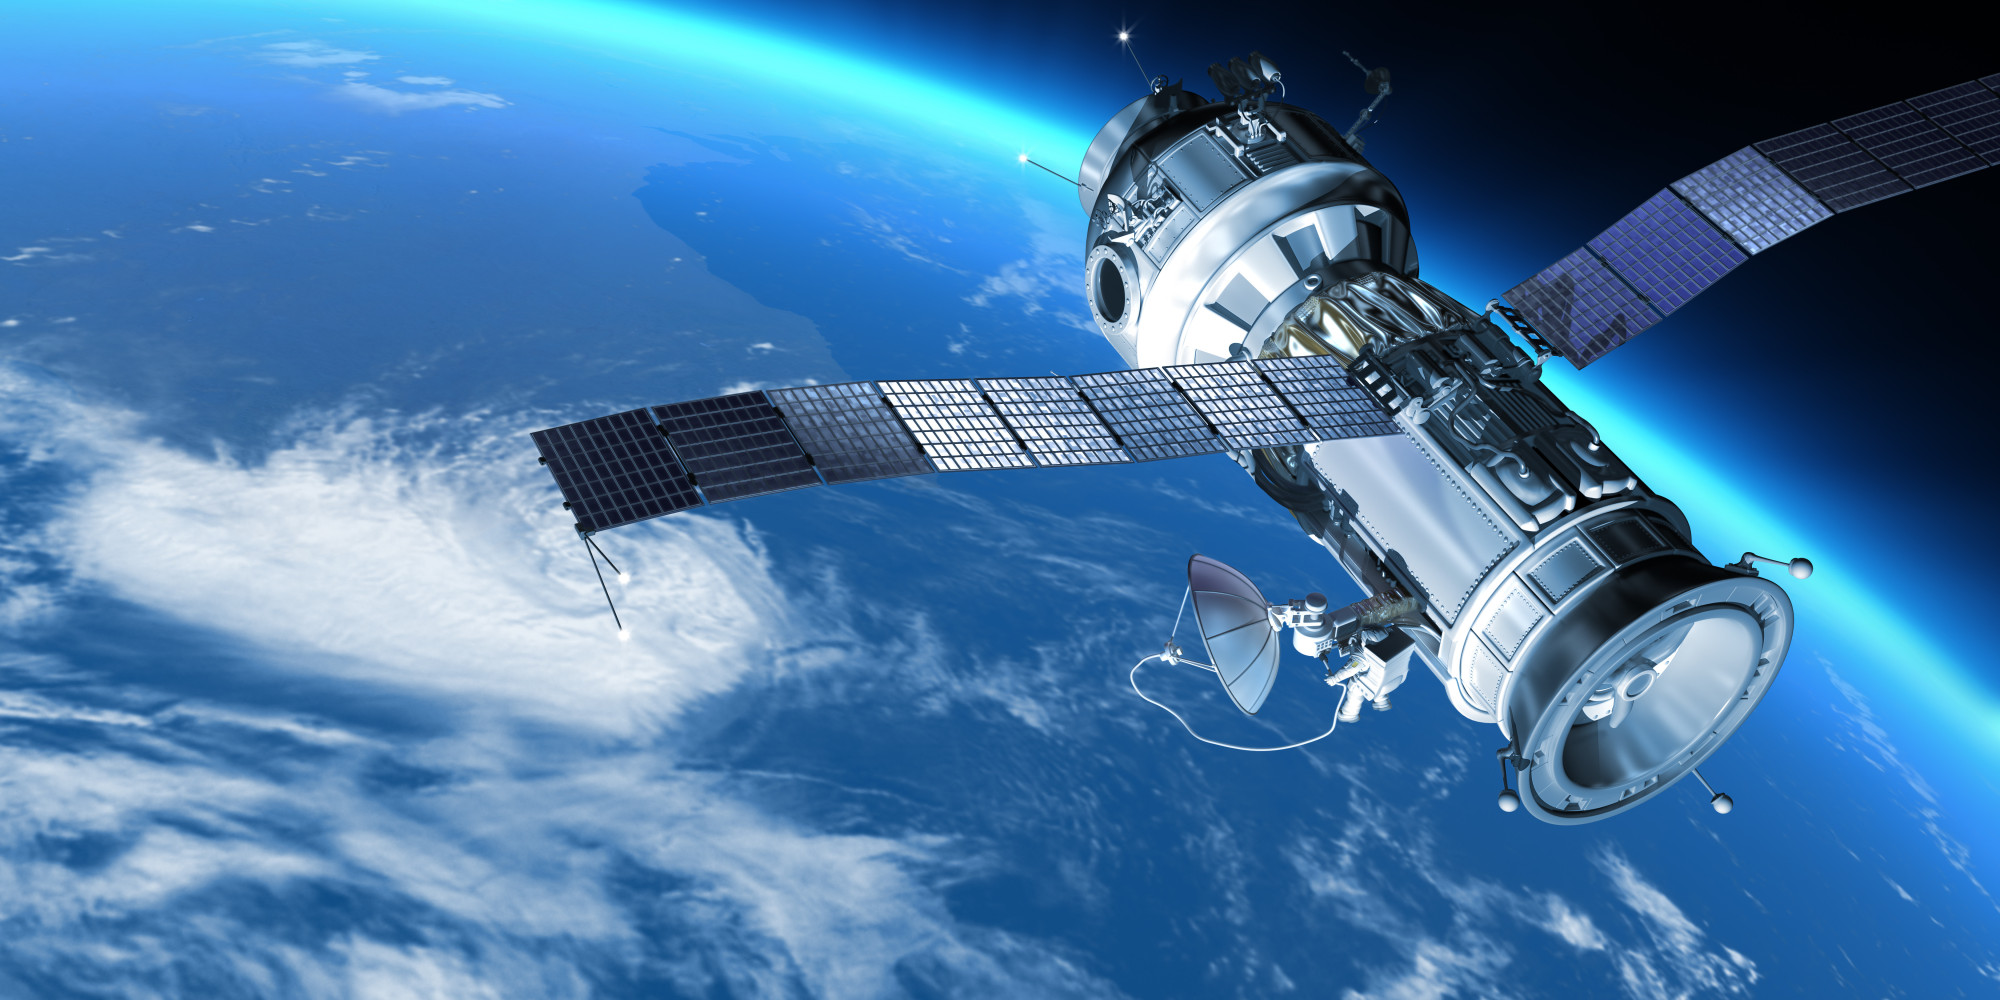
\includegraphics[width=0.5\textwidth]{./fig/Satellite.jpg}
\pause
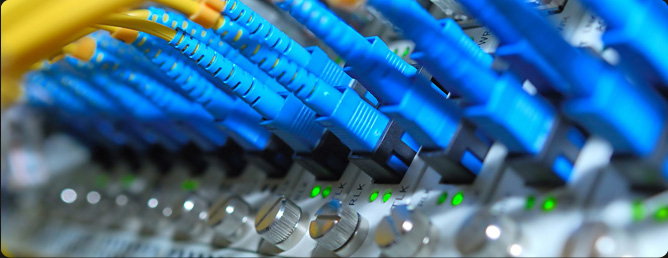
\includegraphics[width=0.5\textwidth]{./fig/internet.jpg}\\
\pause
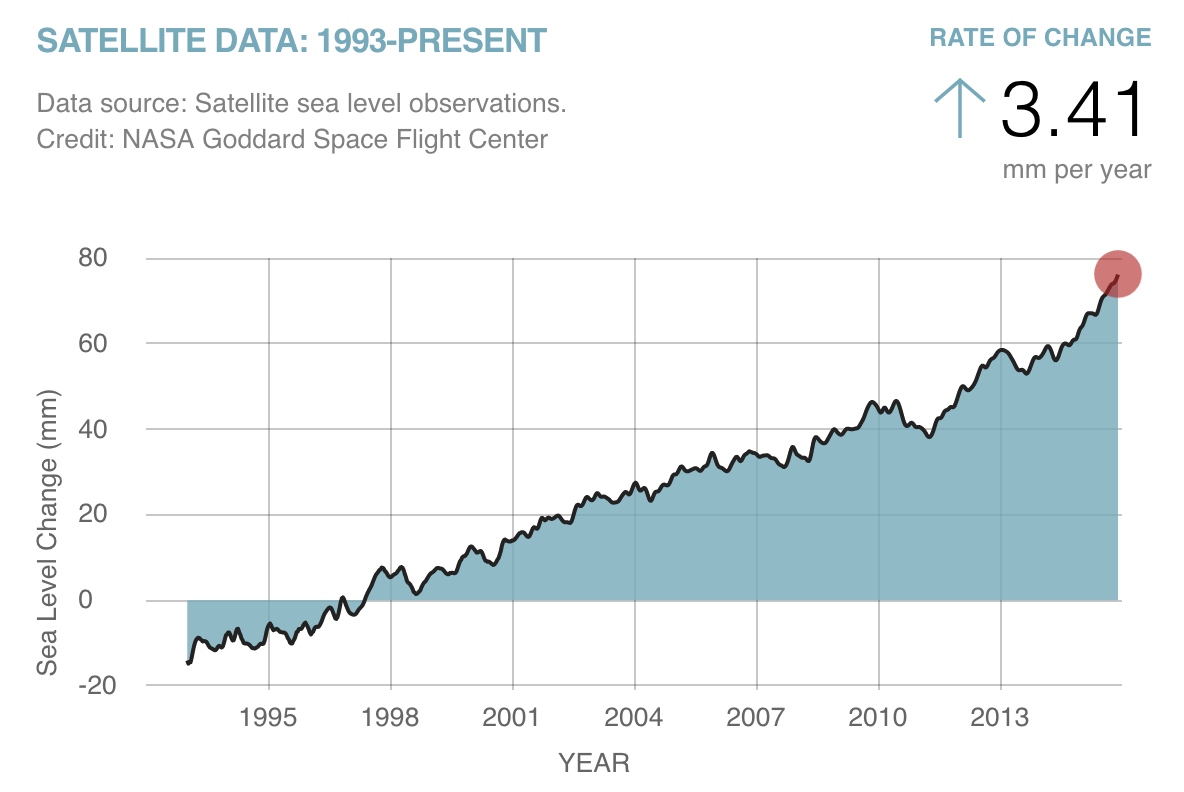
\includegraphics[width=0.5\textwidth]{./fig/sea_level.png}


\end{frame}

%%%%%%%%%%%%%%%%%%%%%
\begin{frame}
\frametitle{What is the subject of "Data science" ?}
\begin{alertblock}{}
Can we extract knowledge, make some predictions, determine a "model" using this large
amount of data ?
\end{alertblock}
\pause
\begin{figure}
\begin{tikzpicture} [
	auto,
	node distance = 1cm]
	\node(H0) [anchor=east]{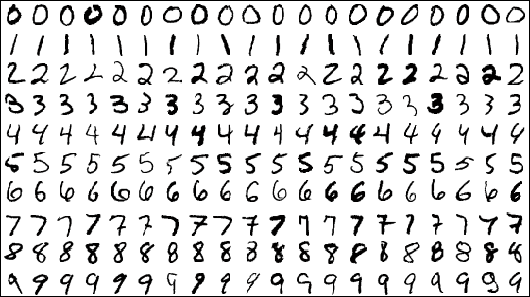
\includegraphics[width=0.4\textwidth]{./fig/mnistExamples.png}};
	\node(H1) [right of =  H0, xshift = .4\textwidth]  
	{Digit \newline $\in \{0,\ldots,9\}$};
	\node(legend) [below of = H0,yshift=-4ex]{Base of images};
	\draw [very thick, ->] (H0)--(H1);
\end{tikzpicture}
\end{figure}
\pause
\begin{itemize}
\item From high dimensional data (thousands to millions dimensions) to reduced dimensional data (less than 100)
\item From disorganized data to comprehensive information
\item \alert{Can we teach a machine how to do that ?}
\end{itemize}

\end{frame}
%%%%%%%%%%%%%%%%%%%%%%%%%
\begin{frame}
\frametitle{Two classes of problems in datascience}
\begin{enumerate}
\item \alert{Regression}: Determination of a quantitative variable from a set of data
\begin{itemize}
\item The price of a building from various informations (Surface, ...)
\item A physical value (Temperature, humidity, ...) in the future knowing the past
\item ...
\end{itemize}
\pause
\item \alert{Classification}: Determination of a class (a label) 
\begin{itemize}
\item A digit from a image
\item Identification of the content of an image
\item ...
\end{itemize}
\end{enumerate}
\end{frame}
%%%%%%%%%%%%%%%%%%%%%%%%%%%
\begin{frame}
\frametitle{Two modes of "learning"}

\begin{enumerate}
\item \alert{Supervised learning}: we have a set of data with examples of what
we want to obtain (some measurements, a survey, ...). We want to derive a general 
rule.
\pause
\item \alert{Unsupervised learning}: we only know the data, we have no examples of
what we want to obtain. We want to extract a "useful" representation of these data, or
some coherent categories.
\begin{itemize}
\item Determine typical behaviors of clients in a supermarket knowing what the have bought.
\end{itemize}
\end{enumerate}
\end{frame}

%%%%%%%%%%%%%%%%%%%%%%%%%%%
\begin{frame}
\frametitle{Outline of the summer school}
\begin{block}{The main idea}
The purpose is to introduce some powerful tools and concepts to 
extract a "meaning" from an amount of data.
\end{block}
\pause
\begin{itemize}
\item Week 1 (J. Brajard, D. Dilmi, G. Moyse) :
\begin{itemize}
\item Basics of Linear Algebra 
\item Some probability and statistics
\item Linear Regression
\item Logistic "Regression"
\item Toward non-linear regression
\end{itemize}
\item Week 2 (G. Contardo, D. Dilmi, F. Balazard):
\begin{itemize}
\item Machine Learning - Neural Networks
\item Deep Learning - Convolutionnal Neural Networks
\item Deep Learning - Recurrent Neural Networks
\item Unsupervised Learning - ACP
\item Unsupervised Learning - K-means, NMF
\end{itemize}
\end{itemize}
\end{frame}

%%%%%%%%%%%%%%%%%%%%%%%%%%%
\begin{frame}
\frametitle{Pratical organization}

\begin{itemize}
\item Morning (9:00 - 12:00) : Lectures in class
\item Afternon (14:00 - 17:00) : Practical work (using \texttt{Python})
\end{itemize}
\end{frame}

\begin{frame}
\frametitle{Some useful online references}
\begin{itemize}
\item Ian GoodFellow et al. (2016) - in presse:\\ \url{http://www.deeplearningbook.org/}
\item MOOC Coursera of Andrew Ng:\\ \url{https://www.coursera.org/learn/machine-learning}
\item nice demonstrator: \\ \url{http://playground.tensorflow.org/}
\item Deep Learning lessons of Yann Lecun (Coll�ge de France) in french:\\
\url{http://www.college-de-france.fr/site/yann-lecun/}
\end{itemize}
\end{frame}

\end{document}